\section{Figures}



\begin{figure}
	\centering
		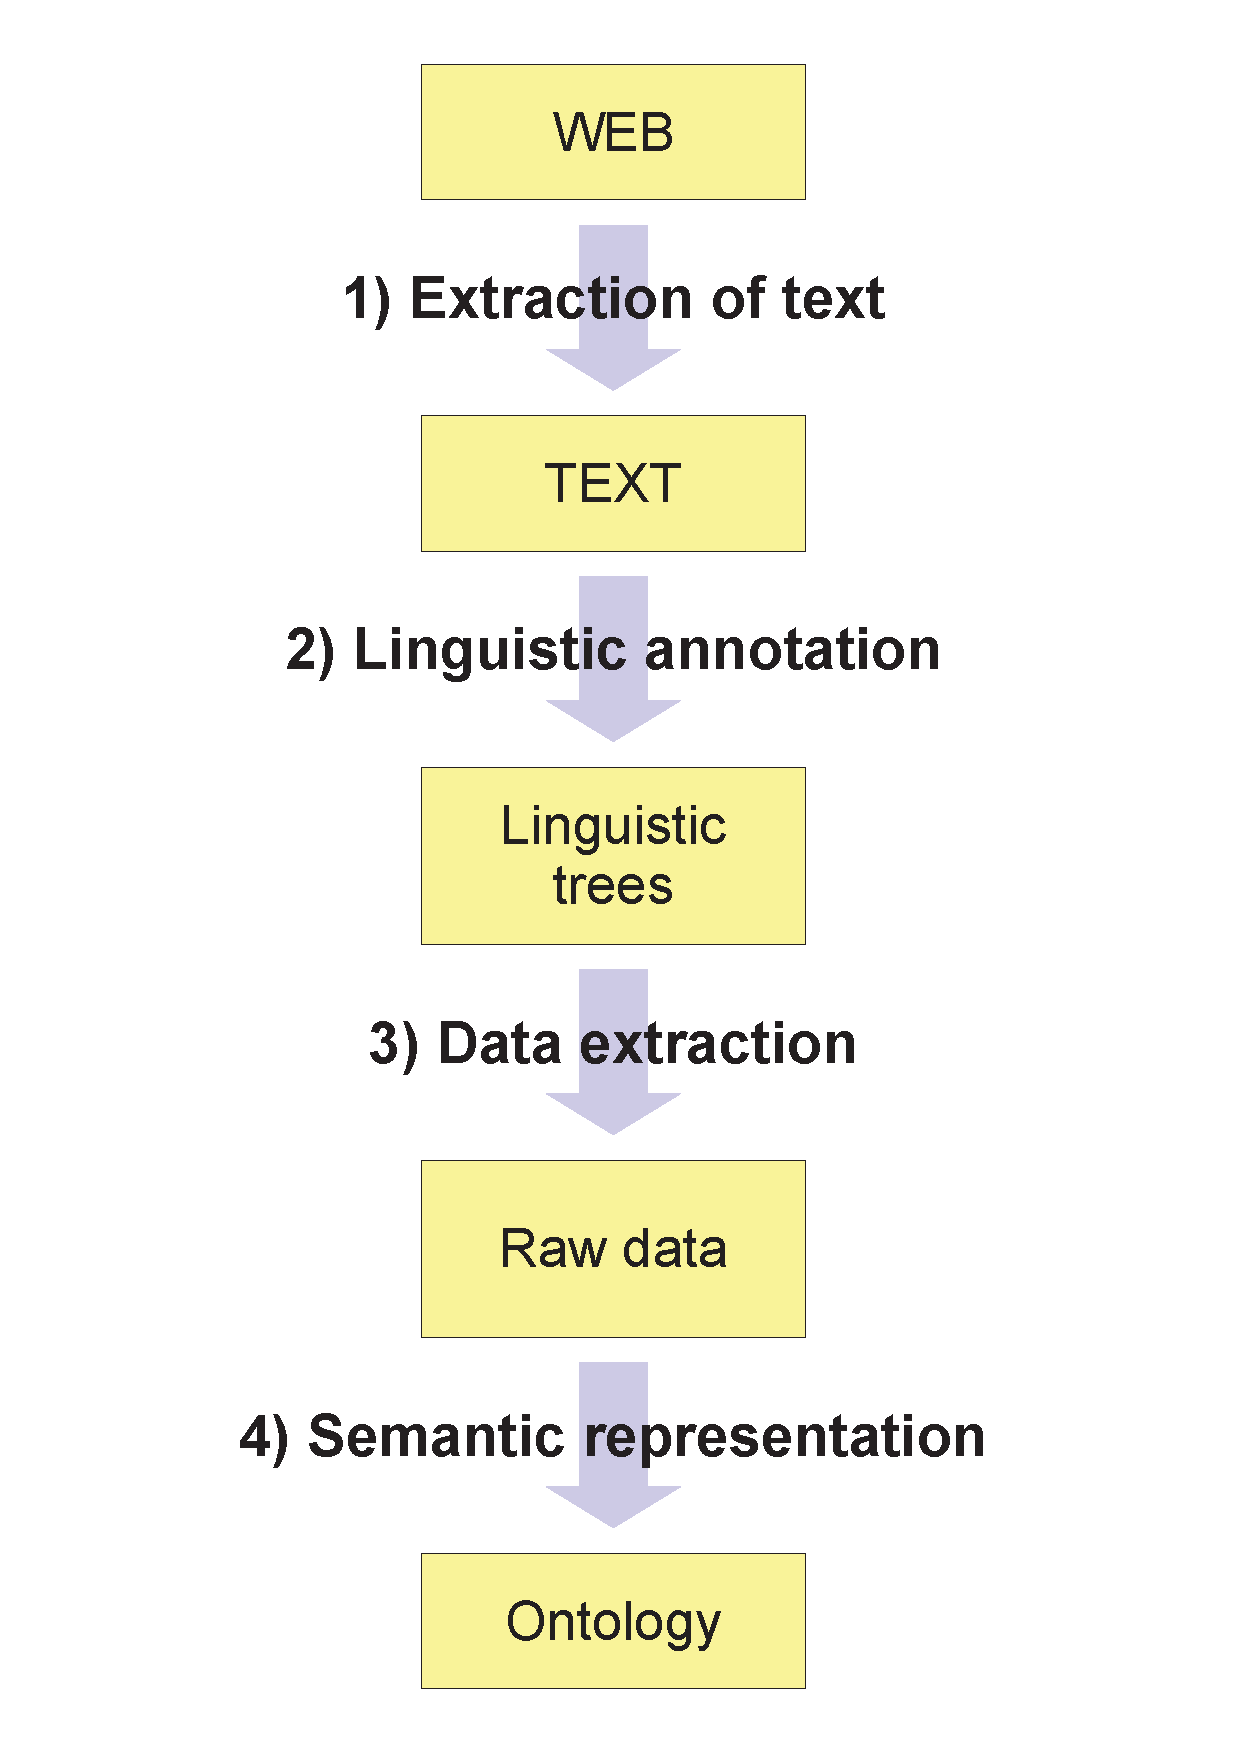
\includegraphics[width=0.2\hsize]{../img/ch3_ap_schema}
	\caption{Schema of the extraction process.}
	\label{fig:ch3_ap_schema}
\end{figure}


\begin{figure}
	\centering
		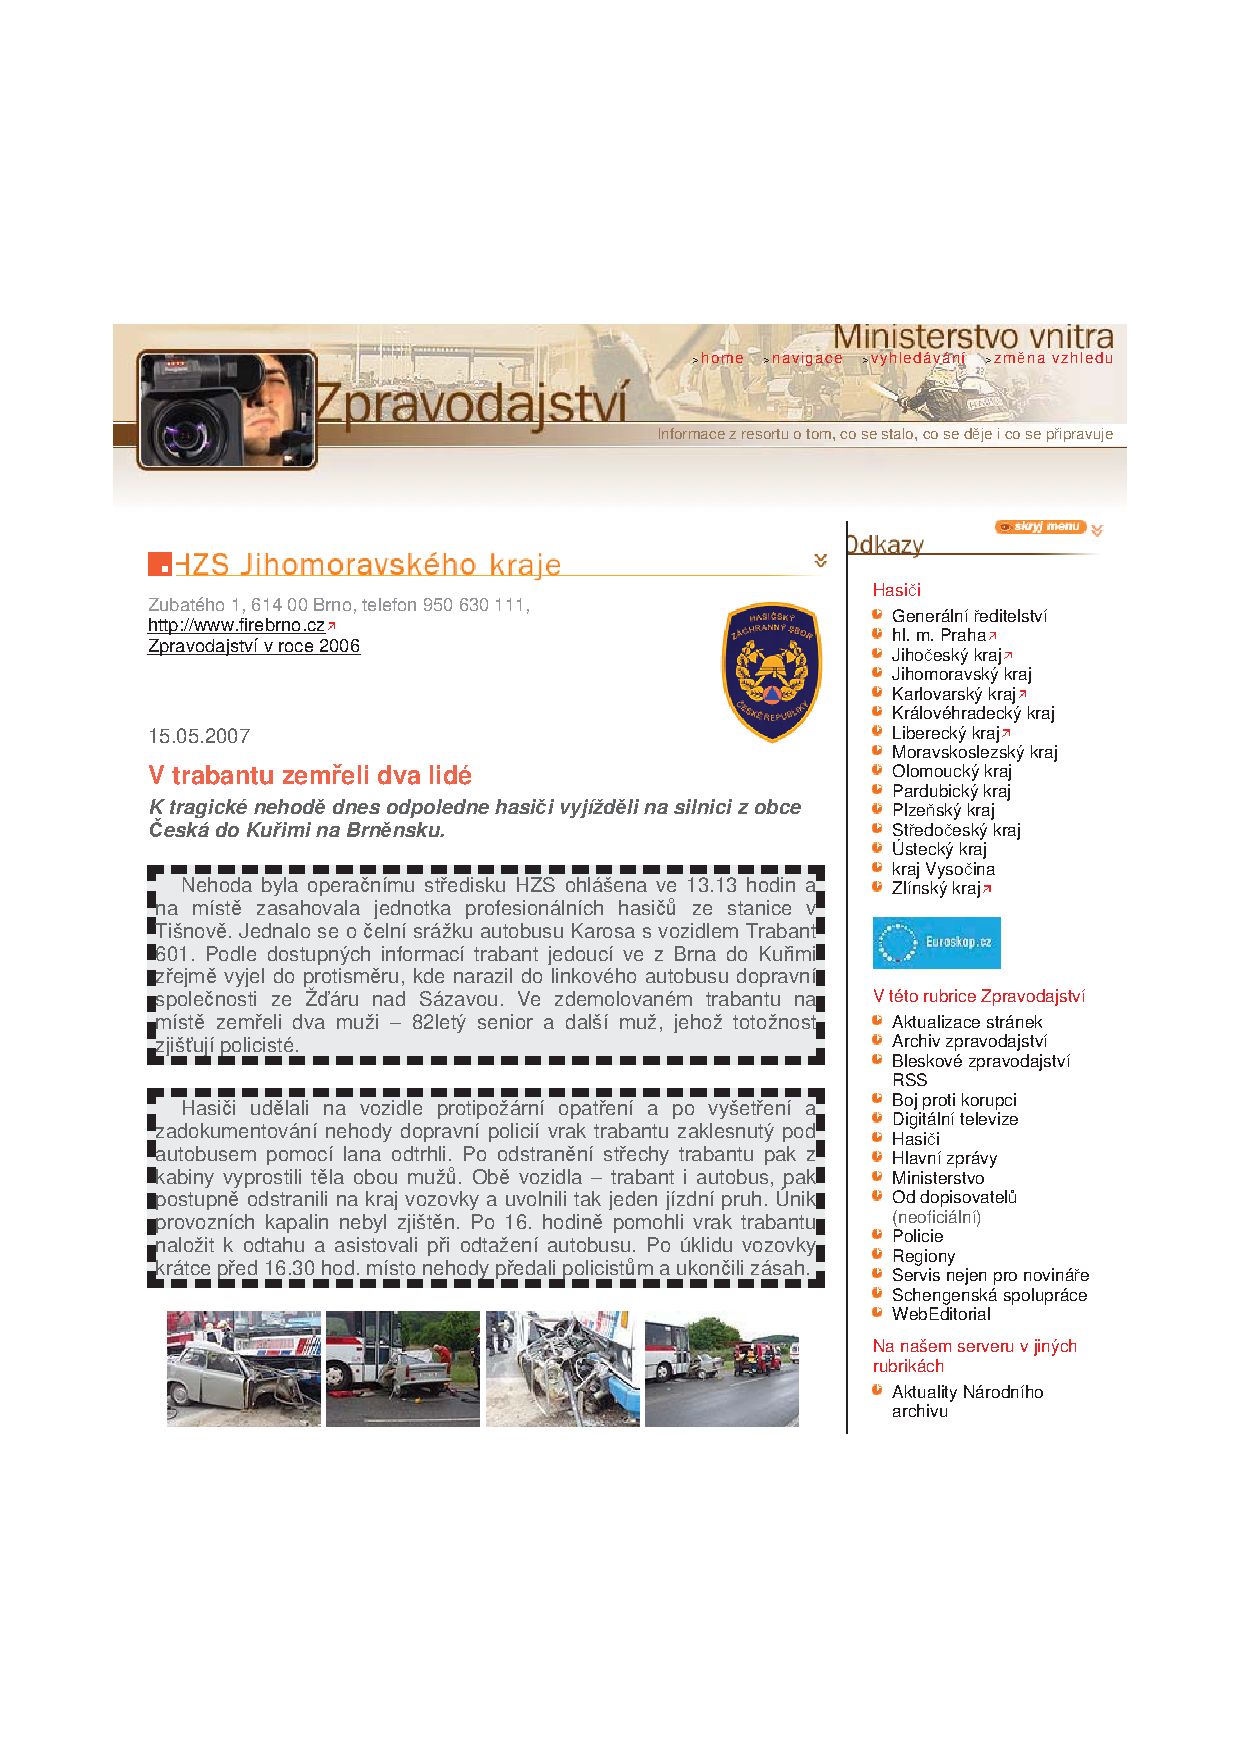
\includegraphics[width=0.5\hsize]{../img/ch3_article}
	\caption{One web page with an accident report.}
	\label{fig:ch3_article}
\end{figure}


\begin{figure}
	\centering
		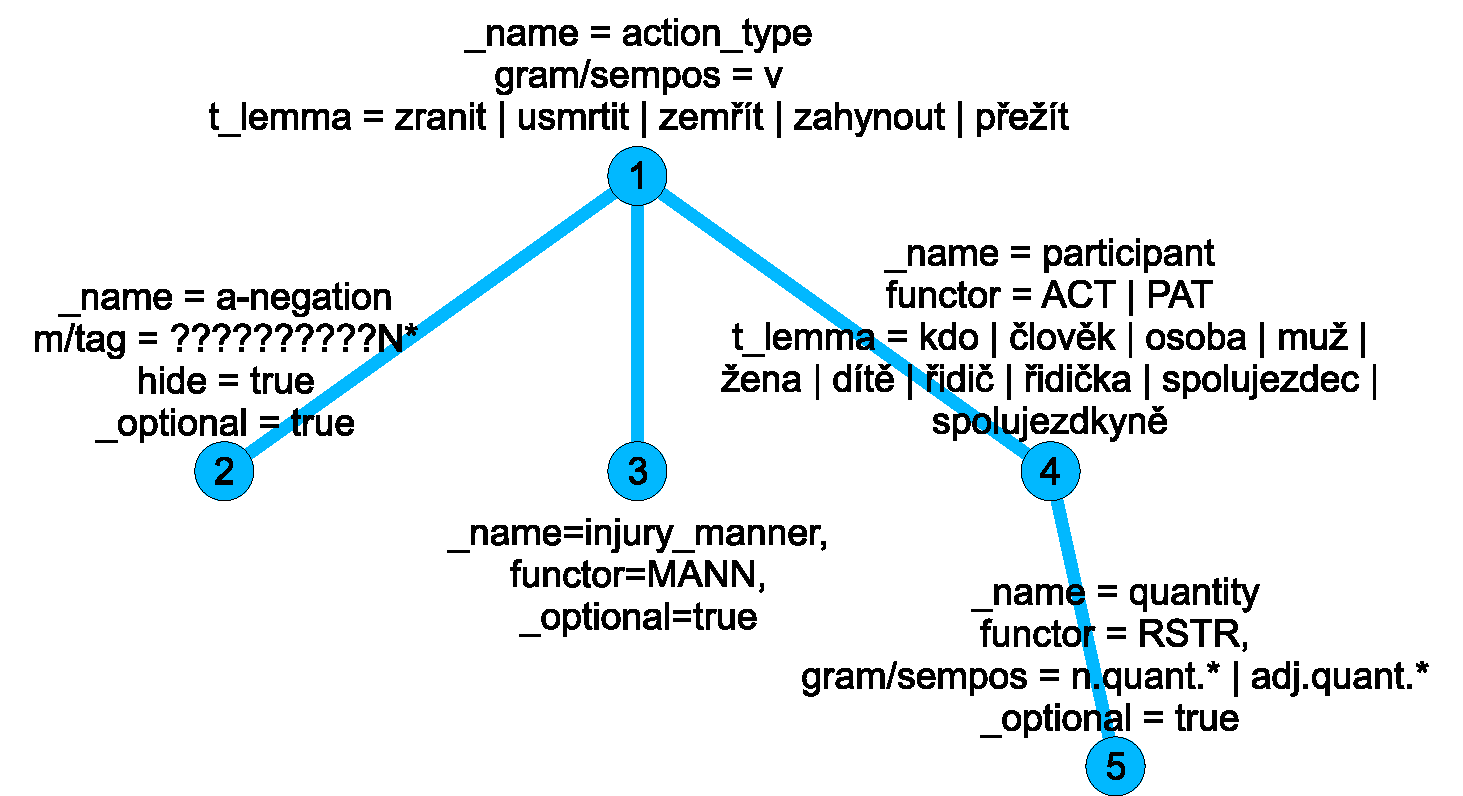
\includegraphics[width=0.5\hsize]{../img/ch3_extract_patern}
	\caption{A manually created extraction rule investigating numbers of injuries and fatalities.}
	\label{fig:ch3_extract_patern}
\end{figure}

\begin{figure}
	\centering
		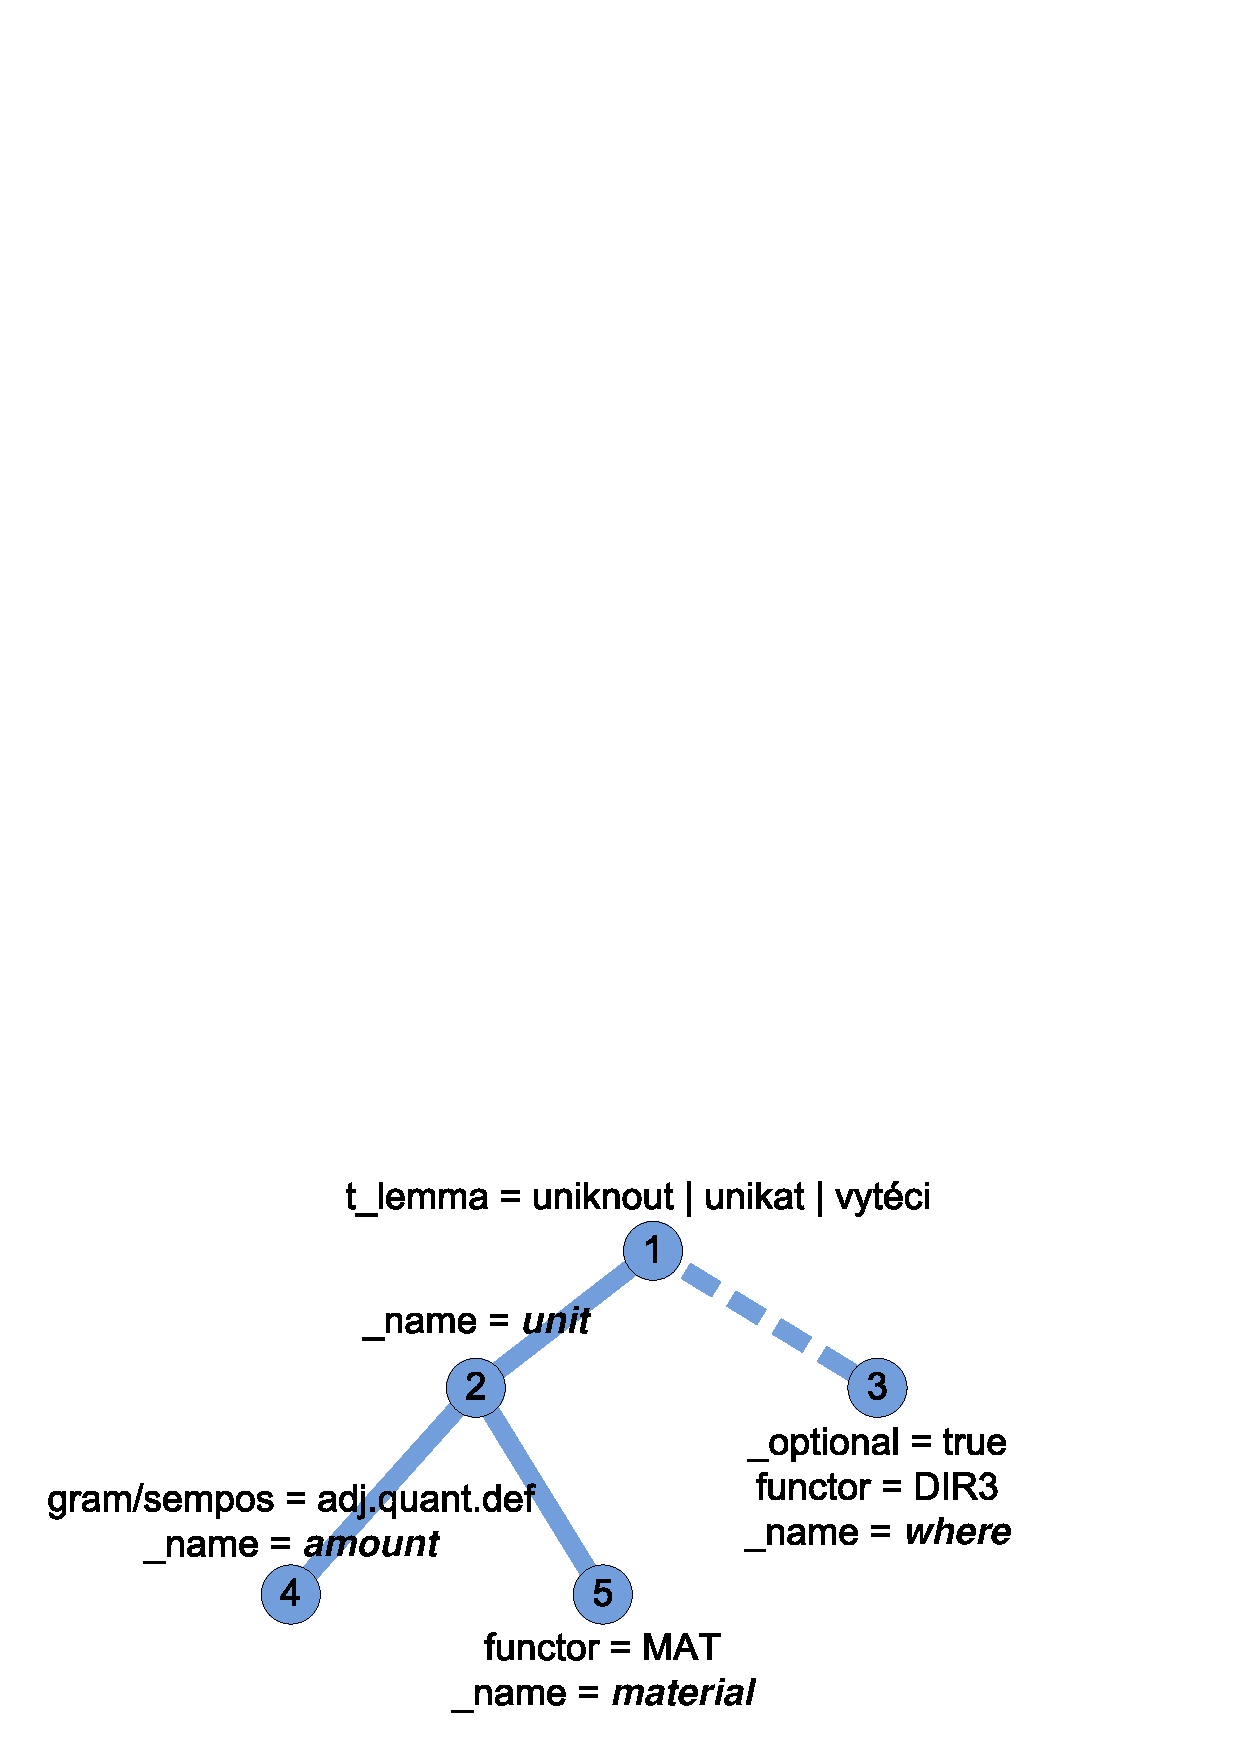
\includegraphics[width=0.5\hsize]{../img/ch3_eenv_extract_patern}
	\caption{A manually created extraction rule investigating dangerous liquids that spilled out into the environment.}
	\label{fig:ch3_eenv_extract_patern}
\end{figure}


\begin{figure}
	\centering
		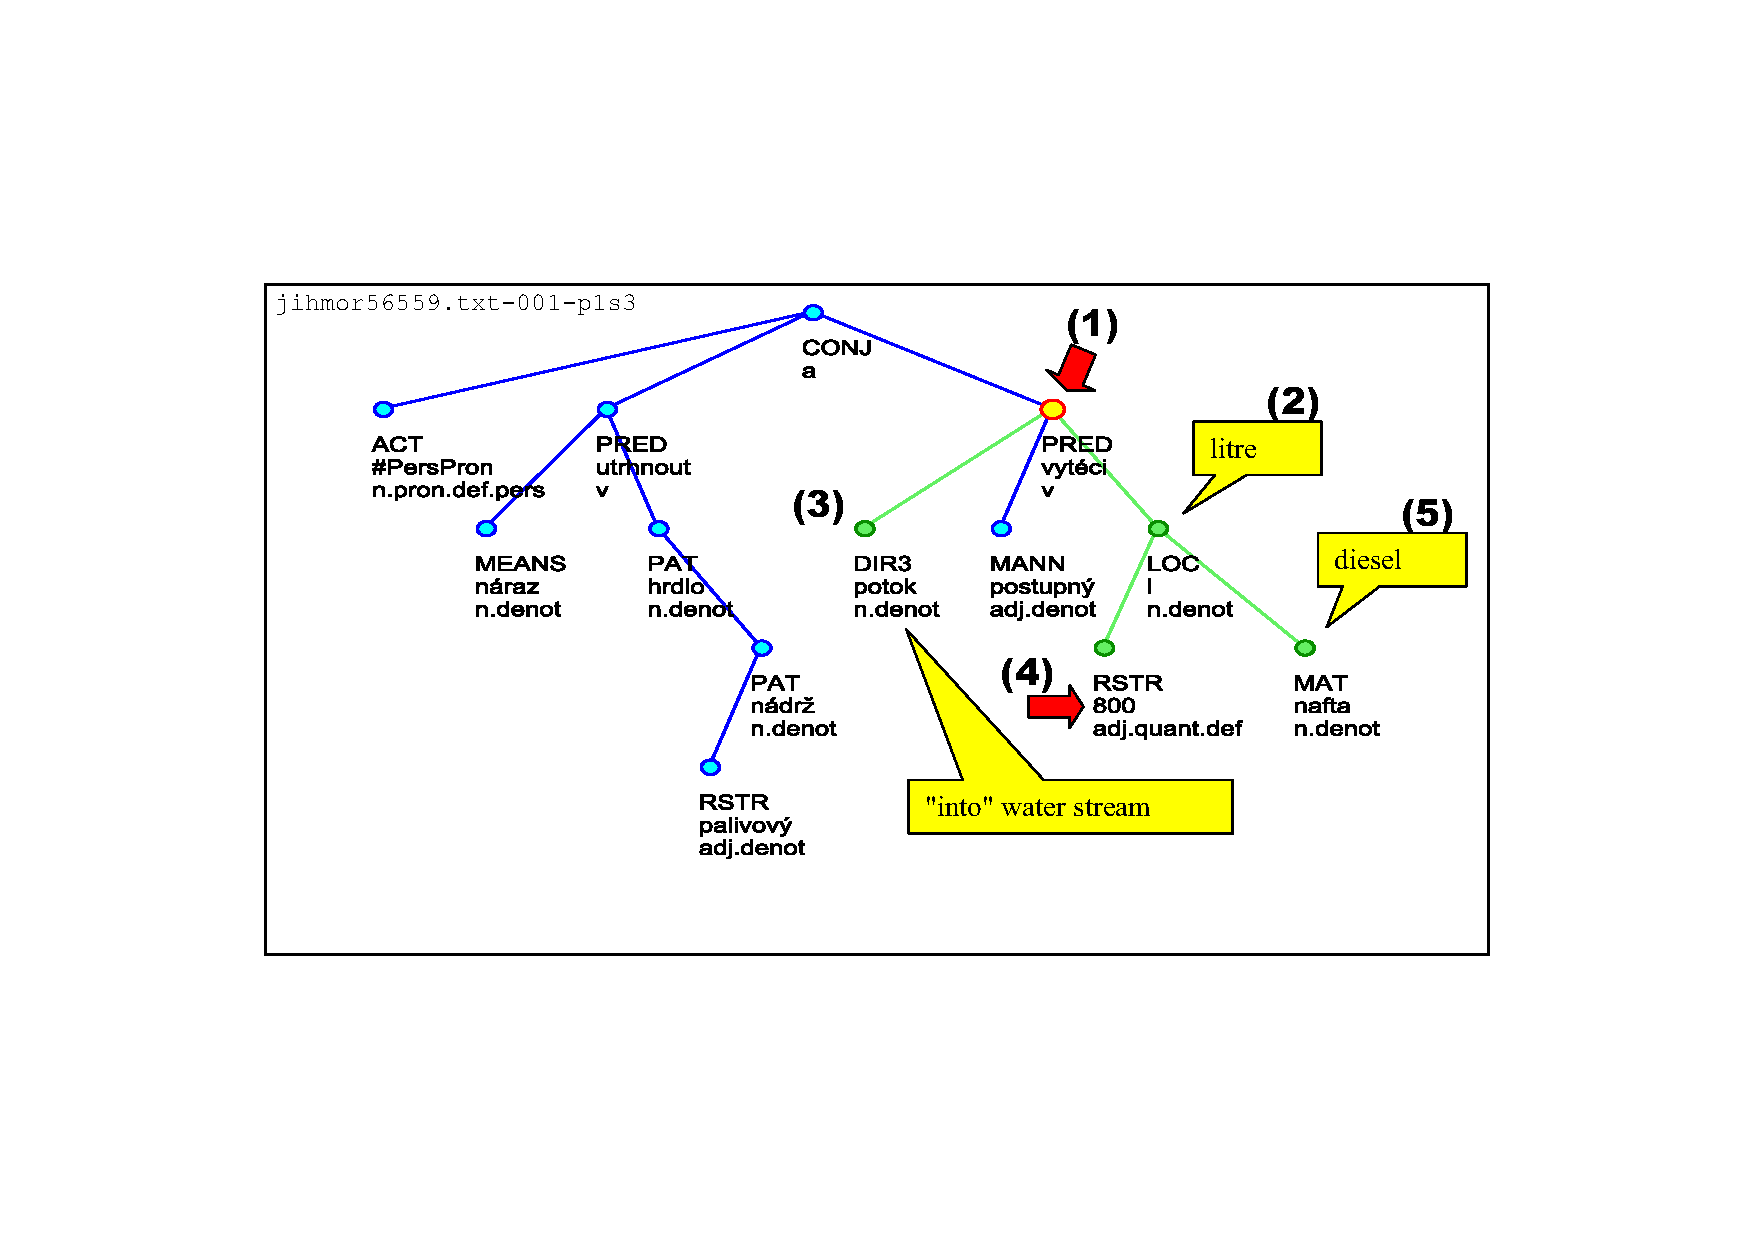
\includegraphics[angle=-90, width=0.6\hsize]{../img/ch3_eenv_matching_tree}
		
Original sentence: 
\emph{``Nárazem se utrhl hrdlo palivové nádrže a do potoka postupně vyteklo na 800 litrů nafty.''}\\
English transcript: 
\emph{``Due to the clash the throat of fuel tank tore off and 800 liters of oil (diesel) has run out to a stream.''}
	\caption{A tree matching with the corresponding extraction rule in Figure~\ref{fig:ch3_eenv_extract_patern}.}
	\label{fig:ch3_eenv_matching_tree}
\end{figure}


\begin{figure}
	\centering
		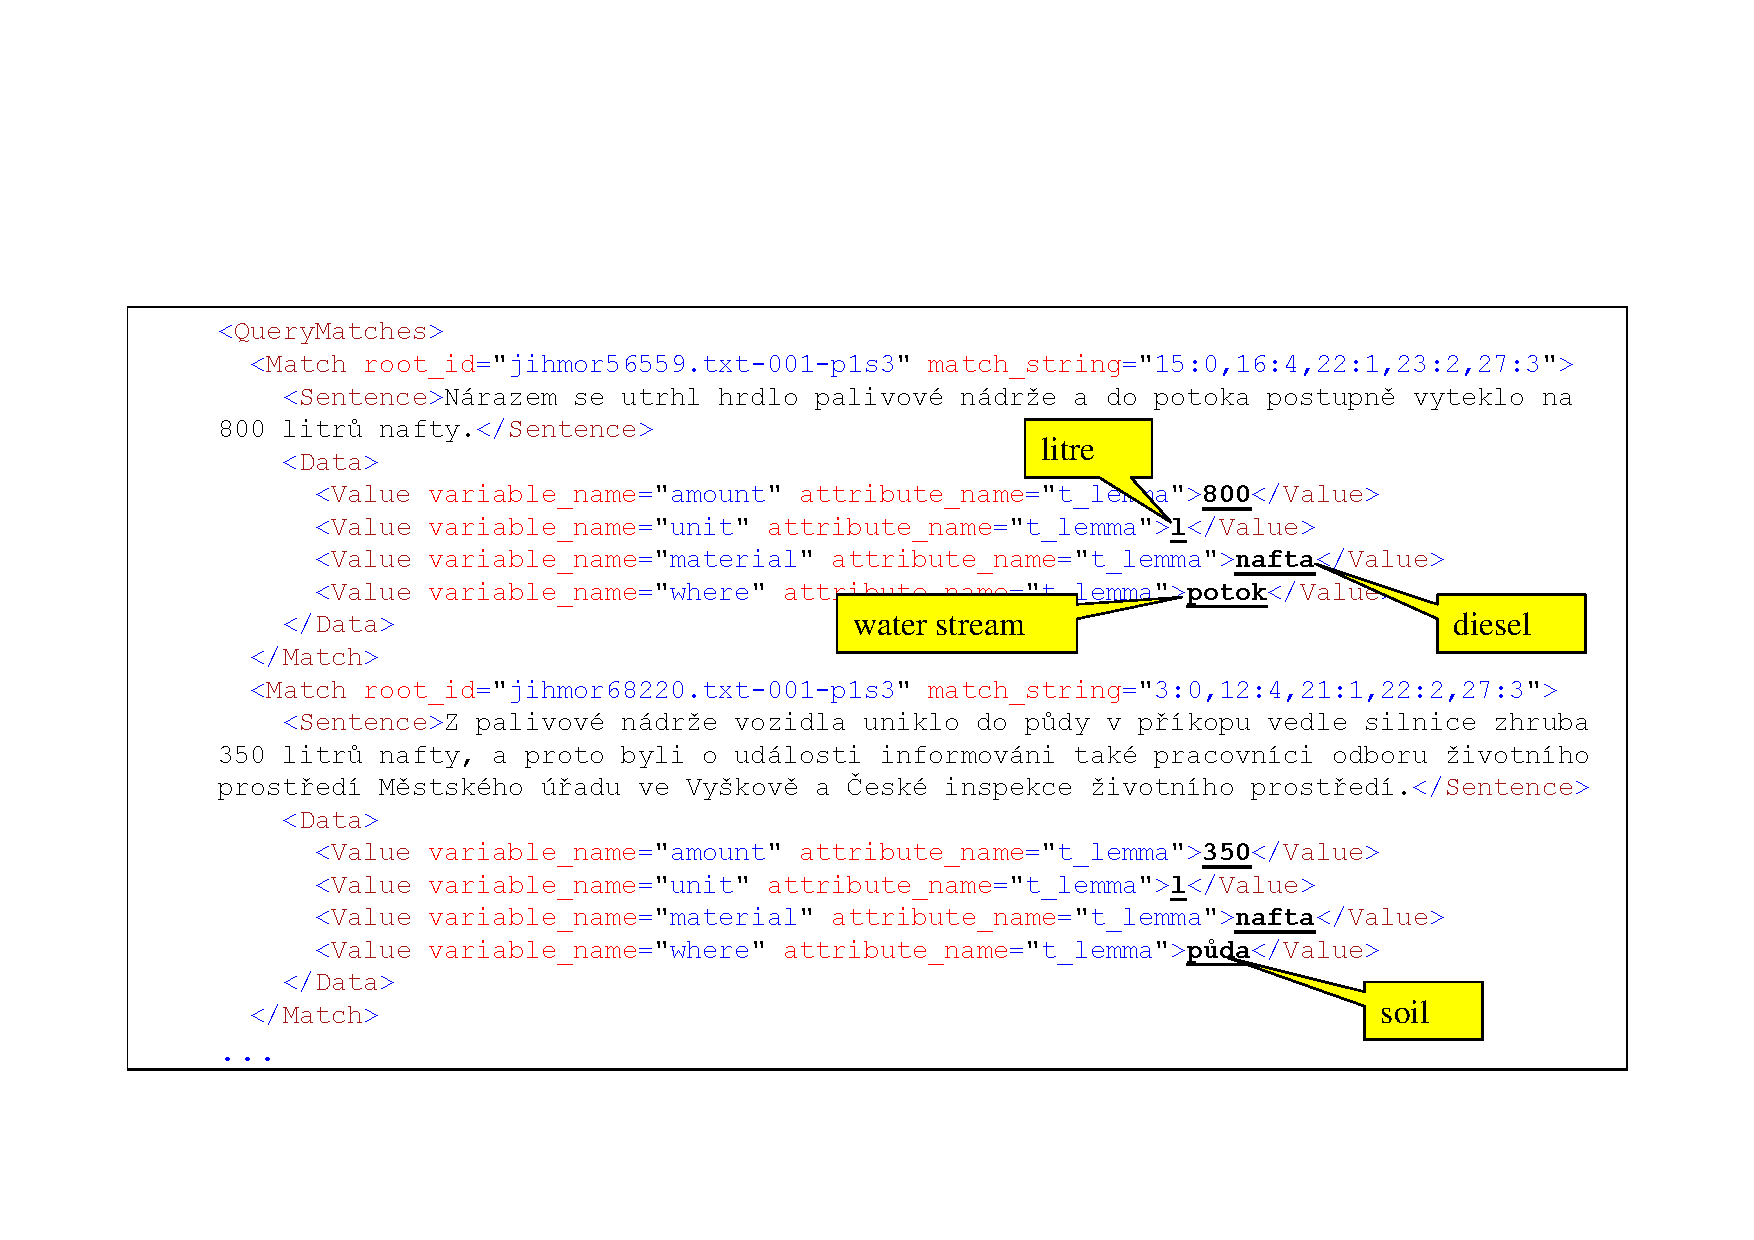
\includegraphics[angle=-90, width=0.7\hsize]{../img/ch3_eenv_results}
	\caption{\emph{XML} structured output of the SQL select like query corresponding with the extraction rule in Figure~\ref{fig:ch3_eenv_extract_patern} and matching tree in Figure~\ref{fig:ch3_eenv_matching_tree}.}
	\label{fig:ch3_eenv_results}
\end{figure}



\begin{figure}
	\centering
		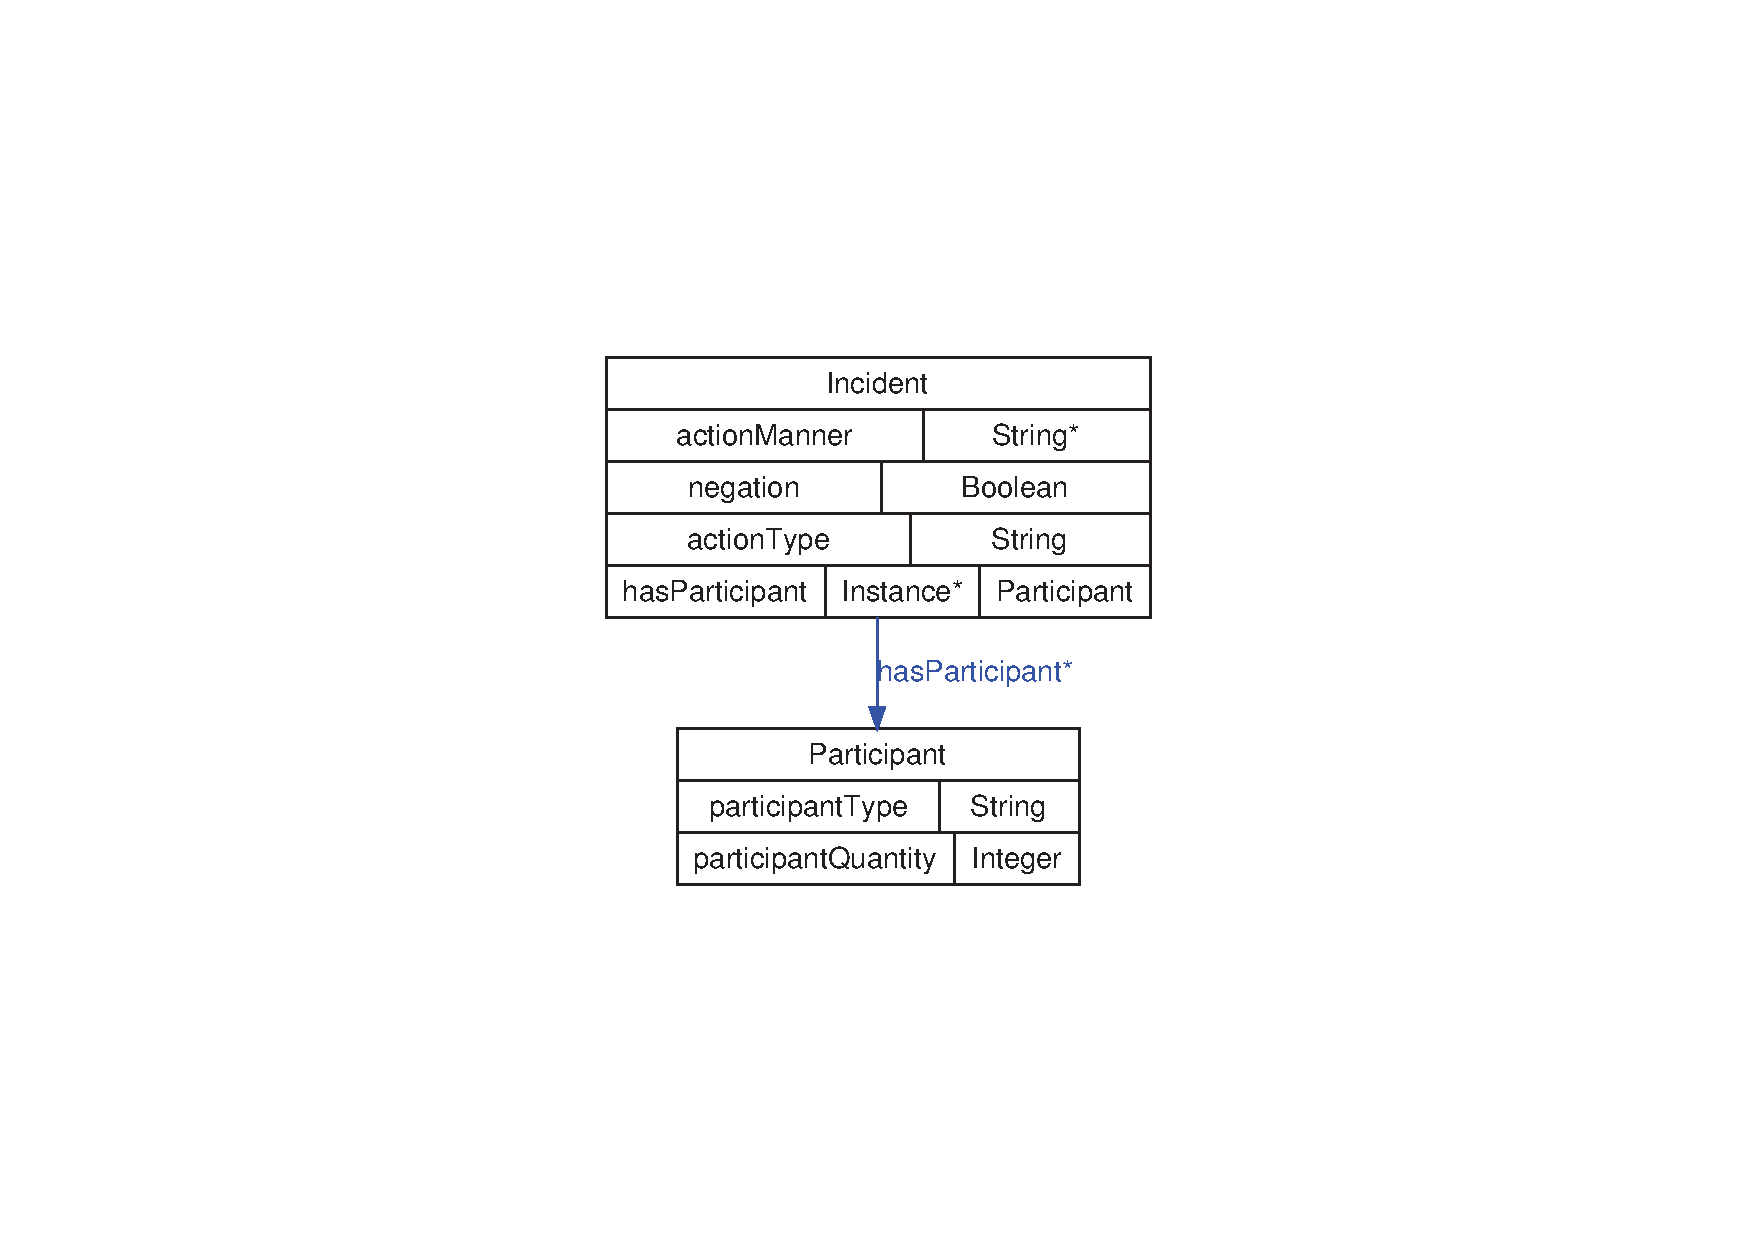
\includegraphics[angle=-90, width=0.3\hsize]{../img/ch3_classes}
	\caption{Schema of the target ontology.}
	\label{fig:ch3_classes}
\end{figure}


\begin{figure}
	\centering
		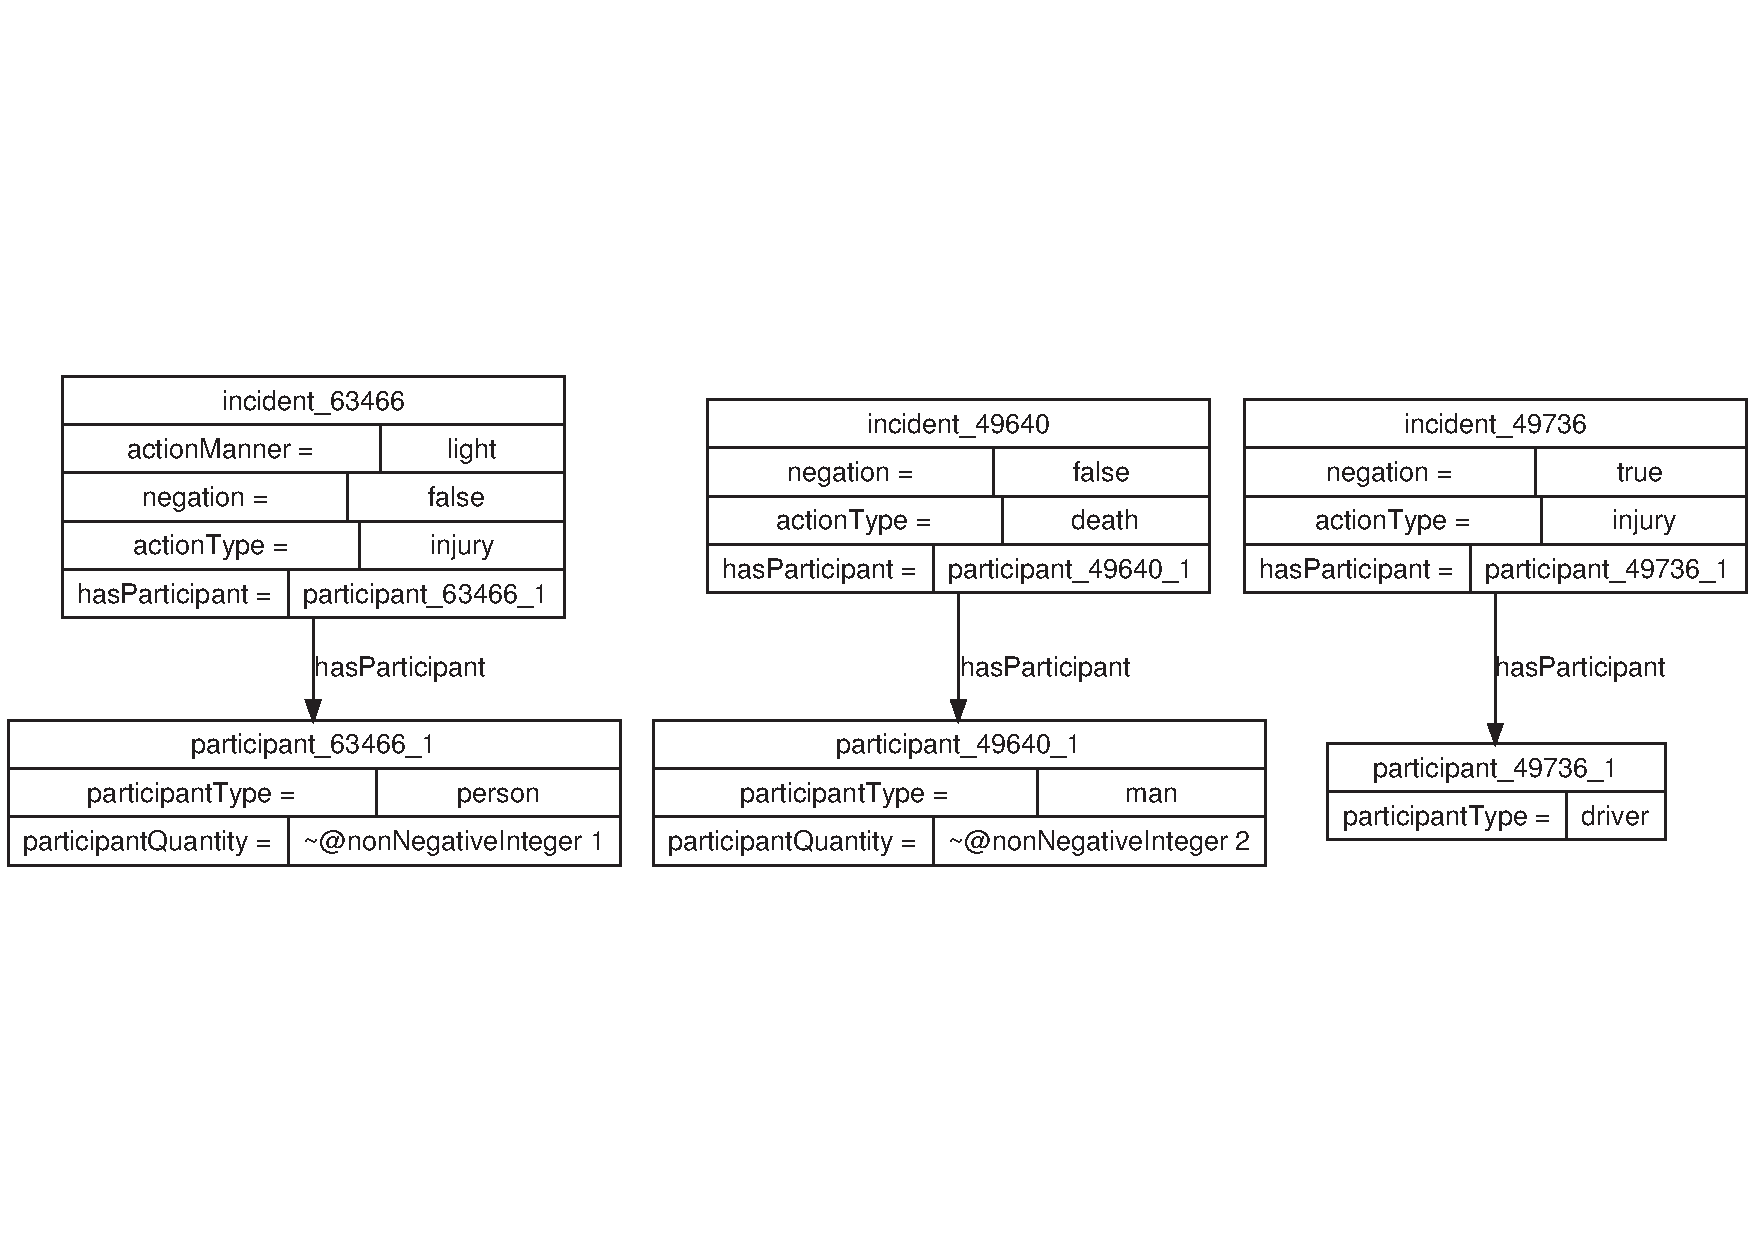
\includegraphics[angle=-90, width=\hsize]{../img/ch3_instances}
	\caption{Extracted instances of the target ontology.}
	\label{fig:instatnces}
\end{figure}


\begin{figure}
	\centering
		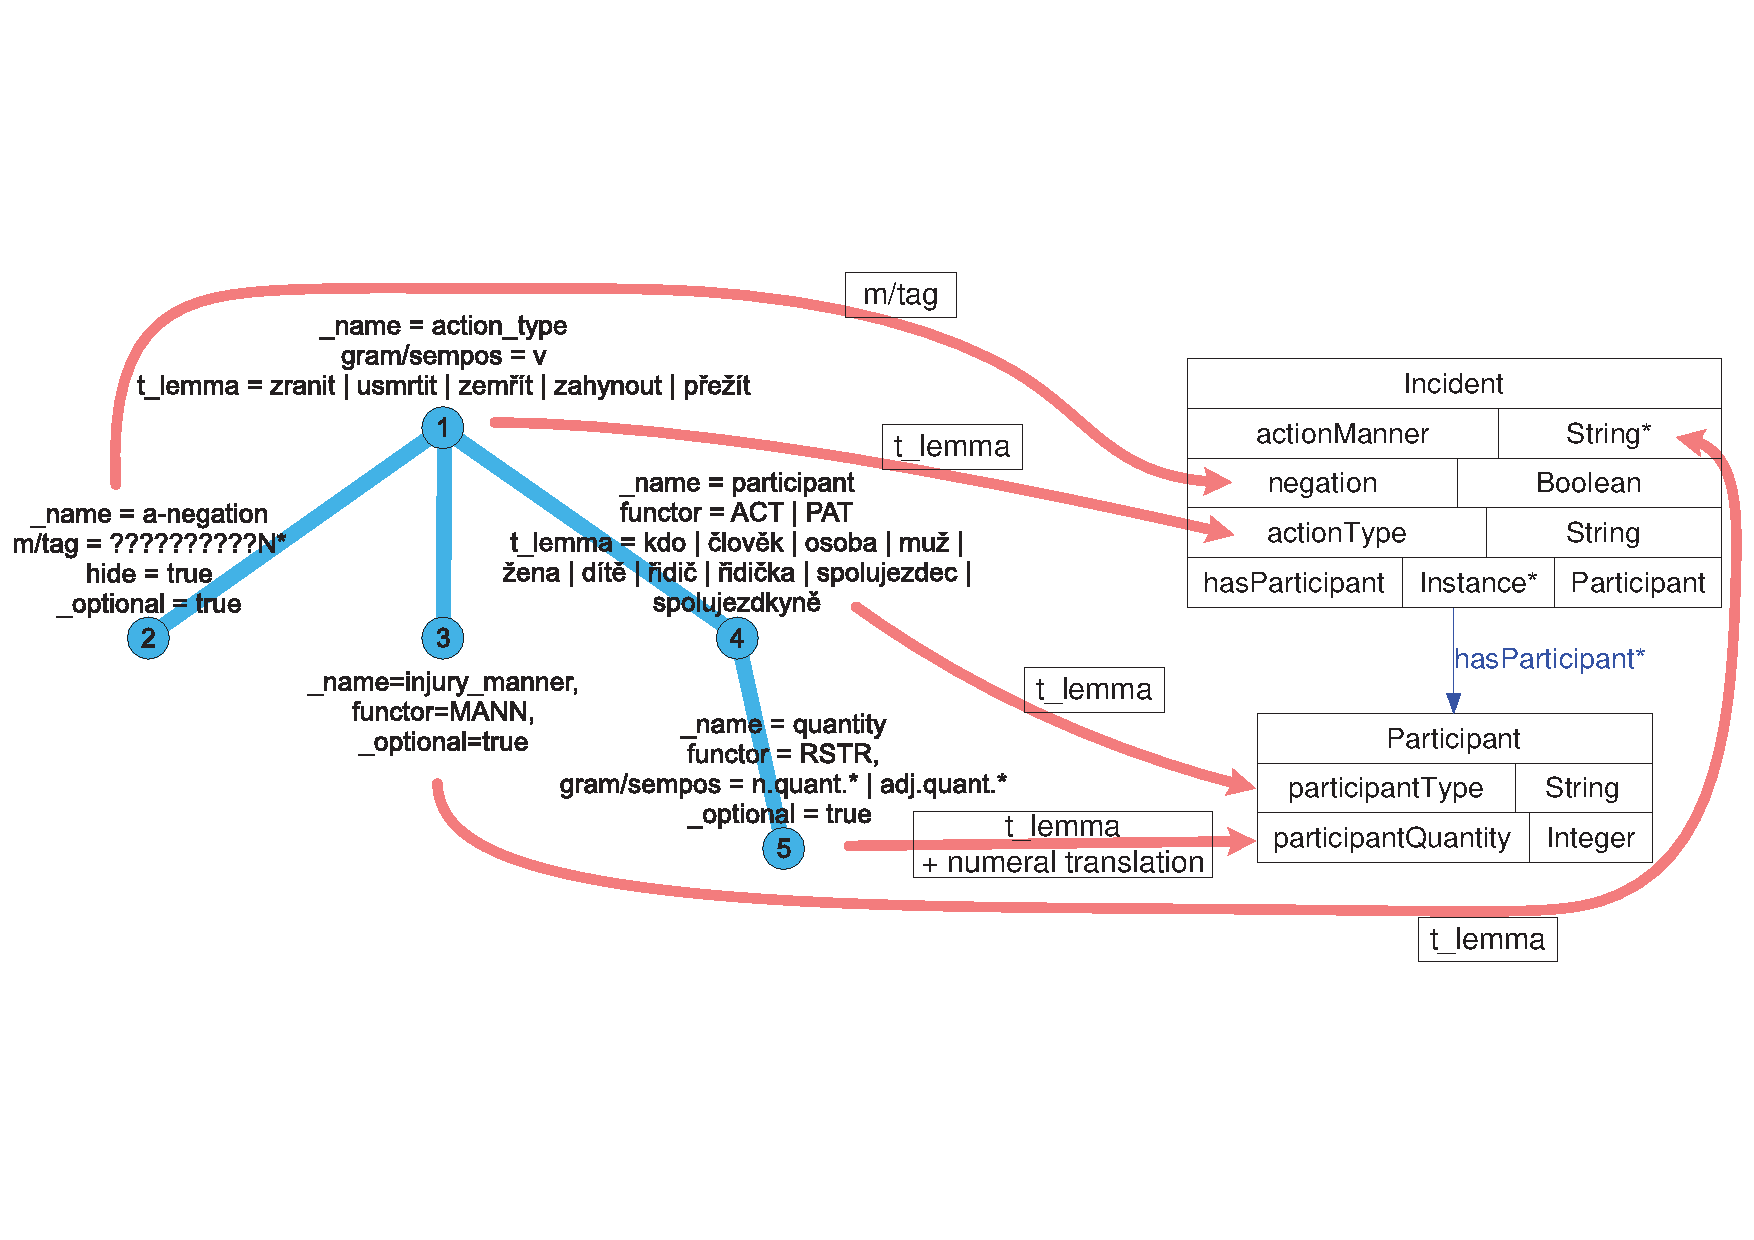
\includegraphics[angle=-90, width=0.9\hsize]{../img/ch3_semantic_interpretation}
	\caption{Semantic interpretation of the extraction rule.}
	\label{fig:ch3_semantic_interpretation}
\end{figure}


\begin{figure}
	\centering
		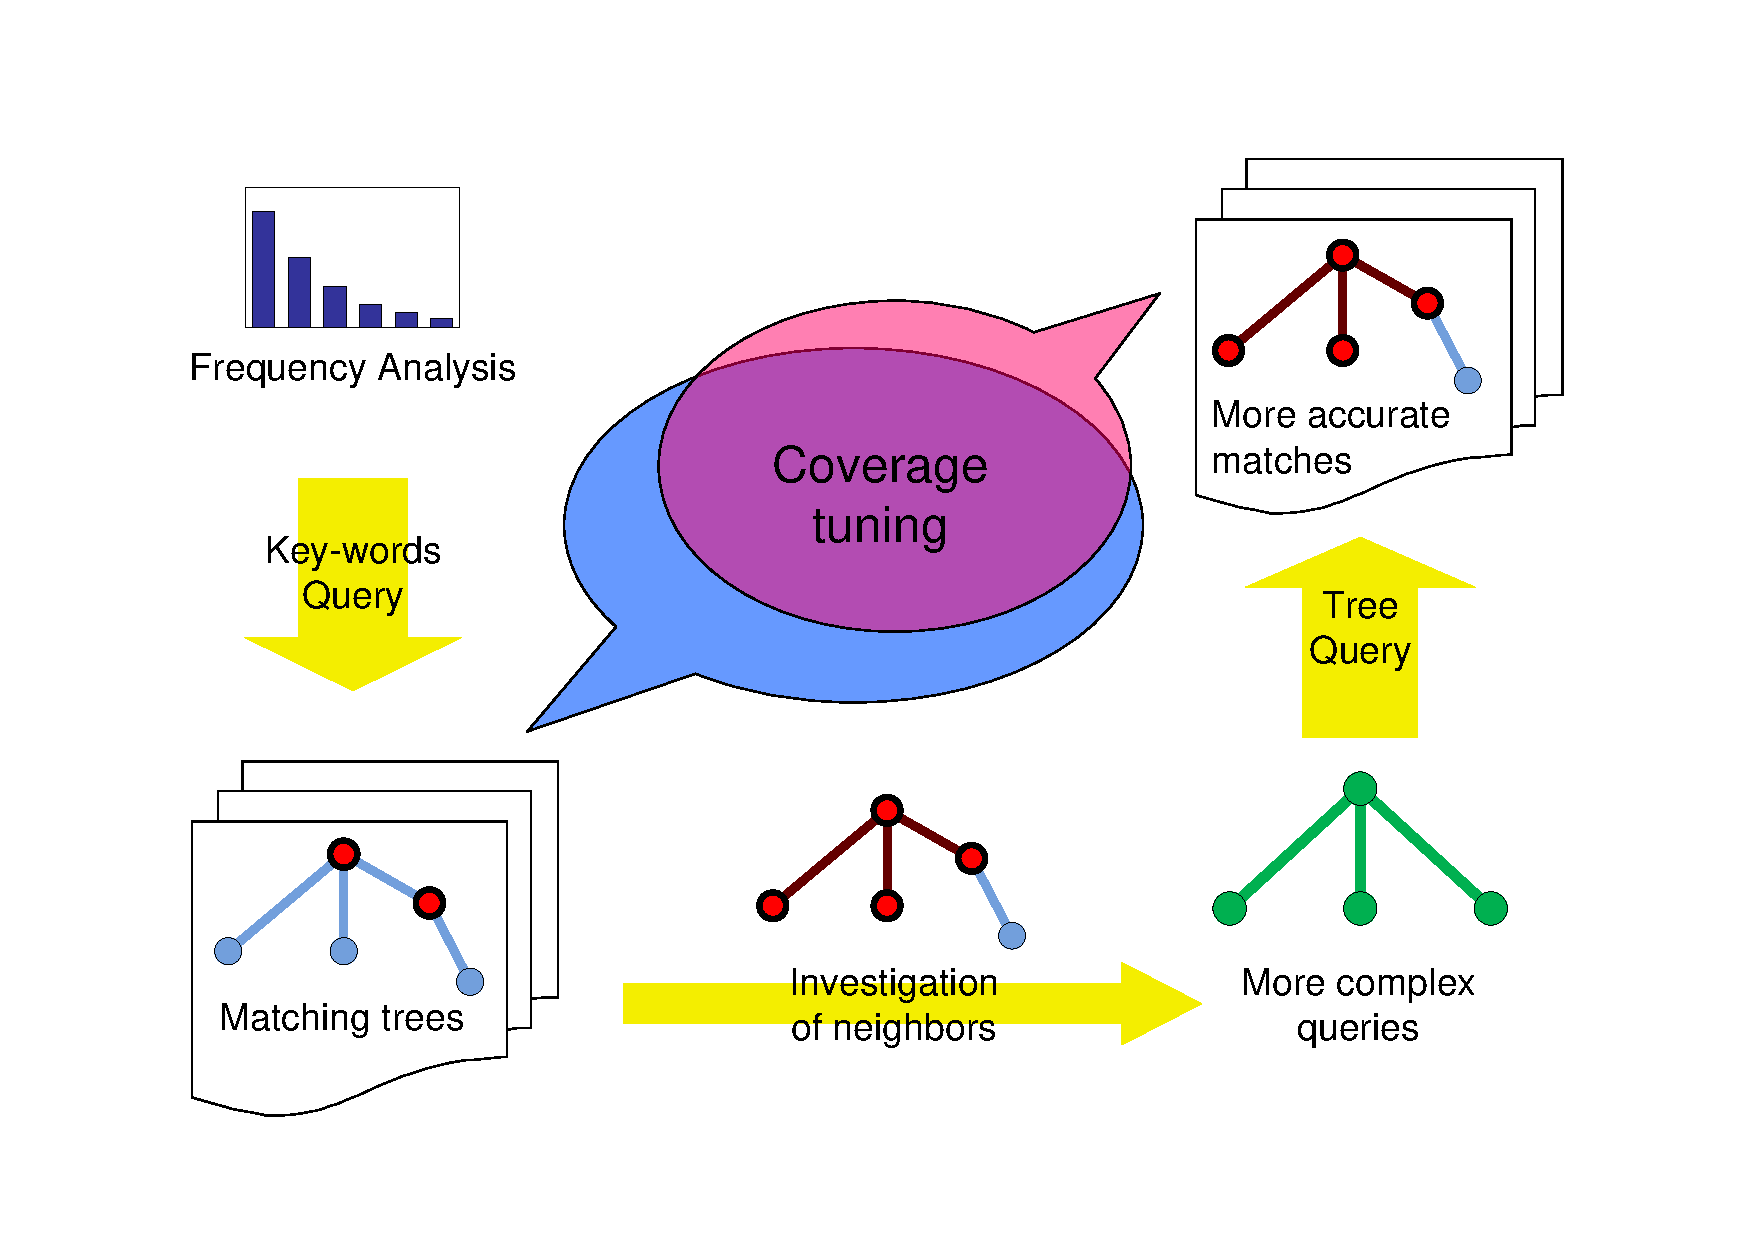
\includegraphics[angle=-90, width=0.5\hsize]{../img/ch3_coverge_tuning}
	\caption{Gradual refinement of an extraction rule.}
	\label{fig:ch3_coverge_tuning}
\end{figure}



\section{Listings}

\begin{listing}
\begin{minted}[linenos,
               frame=lines]{perl}

my @injure_verbs = ("zranit", "usmrtit", "zemřít", "zahynout", "přežít");

sub print_injured {
	if ($this->{gram}{sempos} eq "v") {
		foreach my $v (@injure_verbs) {
			if ($this->{t_lemma} eq $v ) {
				#action type
				print "<action type=\"" . $this->{t_lemma} . "\">";

				#sentece
				print "<sentece>" . PML_T::GetSentenceString($root) . "</sentece>";
				print "<sentece_id>" . $root->{id} . "</sentece_id>";
				
				#negation
				if (test_negation($this)) {
					print "<negation>true</negation>" ;					
				} else {
					print "<negation>false</negation>" ;										
				}
								
				#manner of injurance
				my @mans = find_node_by_attr_depth($this, 0, 'functor', '^MANN');
				if (@mans) {
					foreach my $m (@mans) {
						print "<manner>"; 
						print $m->{t_lemma};
						print "</manner>"; 
					};
				}
				
				#actors and patients
				my @pats = find_node_by_attr($this, 'functor', '^[PA][AC]T');
				@pats = &filter_list(\&test_person, @pats);
				
				foreach my $p (@pats) {
					print "<participant type=\"" . $p->{t_lemma} . "\">";

					#patients count
					my @cnt = find_node_by_attr($p, 'functor', '^RSTR');
					@cnt = &filter_list(\&test_number_lemma, @cnt);
					my $cnt1 = pop(@cnt);
					print "<quantity>" . 
						&test_number($cnt1->{t_lemma}) . 
						"</quantity>" if ($cnt1);
	
					print "<full_string>";
					print_subtree_as_text($p);
					print "</full_string>";

					print "</participant>";
				}
				
				#action end
				print "</action>\n";											
}}}}
\end{minted}
\caption{Procedurally written extraction rule in \emph{btred}.}
\label{lst:btred_rule}
\end{listing}
%%%%%%%%%%%%%%%%%%%%%%%%%%%%%%%%%%%%%%%%%%%%%%%%%%%%%%%%%%%%%%%%%%%%%%%%%%%%%%%%%%%%%



%%%%%%%%%%%%%%%%%%%%%%%%%%%%%%%%%%%%%%%%%%%%%%%%%%%%%%%%%%%%%%%%%%%%%%%%%%%%%%%%%%%%%
\begin{listing}
\begin{minted}[linenos,
               frame=lines]{sparql}

SELECT ?action ?participant ?participant_type ?quantity
WHERE {
	?action rdf:type :Incident;
		:actionType "death";
		:negation false;
		:hasParticipant ?participant.
	?participant :participantType ?participant_type.
	OPTIONAL {
		?participant :participantQuantity ?quantity.
	}
}
\end{minted}
\caption{\emph{SPARQL} query that summarizes fatalities of particular incidents.}
\label{lst:sparql_aggregation}
\end{listing}
%%%%%%%%%%%%%%%%%%%%%%%%%%%%%%%%%%%%%%%%%%%%%%%%%%%%%%%%%%%%%%%%%%%%%%%%%%%%%%%%%%%%%



%%%%%%%%%%%%%%%%%%%%%%%%%%%%%%%%%%%%%%%%%%%%%%%%%%%%%%%%%%%%%%%%%%%%%%%%%%%%%%%%%%%%%
\begin{listing}
\begin{minted}[linenos,
               frame=lines]{xml}
<injured_result>
	<action type="zranit">
		<sentece>
			Při požáru byla jedna osoba lehce zraněna -- jednalo se
			o majitele domu, který si vykloubil rameno.
		</sentece>
		<sentece_id>T-vysocina63466.txt-001-p1s4</sentece_id>
		<negation>false</negation>
		<manner>lehký</manner>
		<participant type="osoba">
			<quantity>1</quantity>
			<full_string>jedna osoba</full_string>
		</participant>
	</action>
	<action type="zemřít">
		<sentece>
			Ve zdemolovaném trabantu na místě zemřeli dva muži -- 82letý
			senior a další muž, jehož totožnost zjišťují policisté.
		</sentece>
		<sentece_id>T-jihomoravsky49640.txt-001-p1s4</sentece_id>
		<negation>false</negation>
		<participant type="muž">
			<quantity>2</quantity>
			<full_string>dva muži</full_string>
		</participant>
	</action>
		<action type="zranit">
		<sentece>čtyřiatřicetiletý řidič nebyl zraněn.</sentece>
		<sentece_id>T-jihomoravsky49736.txt-001-p4s3</sentece_id>
		<negation>true</negation>
		<participant type="řidič">
			<full_string>čtyřiatřicetiletý řidič</full_string>
		</participant>
	</action>
</injured_result>
\end{minted}
\caption{\emph{XML} structured output of the query written in \emph{btred}.}
\label{lst:btred_xml}
\end{listing}
%%%%%%%%%%%%%%%%%%%%%%%%%%%%%%%%%%%%%%%%%%%%%%%%%%%%%%%%%%%%%%%%%%%%%%%%%%%%%%%%%%%%%




%%%%%%%%%%%%%%%%%%%%%%%%%%%%%%%%%%%%%%%%%%%%%%%%%%%%%%%%%%%%%%%%%%%%%%%%%%%%%%%%%%%%%
\begin{listing}
\begin{minted}[linenos,
               frame=lines]{xml}
<QueryMatches>
	<Match root_id="T-vysocina63466.txt-001-p1s4" match_string="2:0,7:3,8:4,11:2">
		<Sentence>
			Při požáru byla jedna osoba lehce zraněna - jednalo se
			o majitele domu, který si vykloubil rameno.
		</Sentence>
		<Data>
			<Value variable_name="action_type" attribute_name="t_lemma">zranit</Value>
			<Value variable_name="injury_manner" attribute_name="t_lemma">lehký</Value>
			<Value variable_name="participant" attribute_name="t_lemma">osoba</Value>
			<Value variable_name="quantity" attribute_name="t_lemma">jeden</Value>
		</Data>
	</Match>
	<Match root_id="T-jihomoravsky49640.txt-001-p1s4" match_string="1:0,13:3,14:4">
		<Sentence>
			Ve zdemolovaném trabantu na místě zemřeli dva muži - 82letý senior
			a další muž, jehož totožnost zjišťují policisté.
		</Sentence>
		<Data>
			<Value variable_name="action_type" attribute_name="t_lemma">zemřít</Value>
			<Value variable_name="participant" attribute_name="t_lemma">muž</Value>
			<Value variable_name="quantity" attribute_name="t_lemma">dva</Value>
		</Data>
	</Match>
	<Match root_id="T-jihomoravsky49736.txt-001-p4s3" match_string="1:0,3:3,7:1">
		<Sentence>Čtyřiatřicetiletý řidič nebyl zraněn.</Sentence>
		<Data>
			<Value variable_name="action_type" attribute_name="t_lemma">zranit</Value>
			<Value variable_name="a-negation" 
			       attribute_name="m/tag">VpYS---XR-NA---</Value>
			<Value variable_name="participant" attribute_name="t_lemma">řidič</Value>
		</Data>
	</Match>
</QueryMatches>
\end{minted}
\caption{\emph{XML} structured output of the SQL select like query. A negation can be detected form the \emph{m/tag} on the line 30.}
\label{lst:select_xml}
\end{listing}
%%%%%%%%%%%%%%%%%%%%%%%%%%%%%%%%%%%%%%%%%%%%%%%%%%%%%%%%%%%%%%%%%%%%%%%%%%%%%%%%%%%%%


%%%%%%%%%%%%%%%%%%%%%%%%%%%%%%%%%%%%%%%%%%%%%%%%%%%%%%%%%%%%%%%%%%%%%%%%%%%%%%%%%%%%%%%%%%%%%%%%%
\section{Linguistic tools for automatic annotation of texts} \label{sec:ling_tools}
%%%%%%%%%%%%%%%%%%%%%%%%%%%%%%%%%%%%%%%%%%%%%%%%%%%%%%%%%%%%%%%%%%%%%%%%%%%%%%%%%%%%%%%%%%%%%%%%%


In this section we will describe the linguistic tools that we have used to produce linguistic annotation of texts. These tools are being developed in the Institute of Formal and Applied Linguistics\footnote{\url{http://ufal.mff.cuni.cz}} in Prague (ÚFAL), Czech Republic. They are publicly available -- they have been published on a CD-ROM under the title PDT 2.0 -- \citealt{biblio:PDT20_CD} (first five tools) and in \citealt{biblio:KlTransformationBasedTectogrammatical2006} (Tectogrammatical analysis). These tools are used as a processing chain and at the end of the chain they produce tectogrammatical \citep{biblio:MiBeAnnotationtectogrammatical2006} dependency trees. The Table~\ref{tab:ling_tools} shows some details about these tools.



\begin{enumerate}
	\item \textbf{Segmentation and tokenization} consists of tokenization (dividing the input text into words and  punctuation) and segmentation (dividing a sequences of tokens into sentences).
	
	\item \textbf{Morphological analysis} assigns all possible lemmas and morphological tags to particular word forms (word occurrences) in the text.
	
	\item \textbf{Morphological tagging} consists in selecting a single pair lemma-tag from all possible alternatives assigned by the morphological analyzer.
	
	\item \textbf{Collins' parser -- Czech adaptation} \citep{biblio:collinshbrt_1999}
		
Unlike the usual approaches to the description of English syntax, the Czech syntactic descriptions are dependency-based, which means, that every edge of a syntactic tree captures the relation of dependency between a governor and its dependent node. Collins' parser gives the most probable parse of a given input sentence.
	
	\item \textbf{Analytical function assignment} assigns a description (\emph{analytical function} -- in linguistic sense) to every edge in the syntactic (dependency) tree.
	
	\item \textbf{Tectogrammatical analysis} \citep{biblio:KlTransformationBasedTectogrammatical2006} produces linguistic annotation at the tectogrammatical level.

%	Tectogrammatical analysis produces linguistic annotation at the tectogrammatical layer, sometimes called “layer of deep syntax”. Annotation of a sentence at this layer is closer to meaning of the sentence than its syntactic annotation and thus information captured at the tectogrammatical layer is crucial for machine understanding of a natural language \citep{biblio:KlTransformationBasedTectogrammatical2006}.
	 
\end{enumerate}





\begin{table}
\centering
\caption{Linguistic tools for machine annotation}
%\renewcommand{\arraystretch}{1.4}
	\begin{tabular}{l|l}
		Name of the tool & Evaluation results (proclaimed by authors) \\[4pt]
		\hline
	Segmentation and tokenization & precision(p): 98,0\%, recall(r): 91,4\% \\[4pt]
	Morphological analysis & 2,5\% unrecognized words\\
	Morphological tagging & 93,0\% of tags assigned correctly \\[4pt]
	Collins' parser -- Czech adaptation & 81,6\% dependencies assigned correctly\\
	Analytical function assignment & precision: 92\% \\[4pt]
	Tectogrammatical analysis & dependencies p:~90,2\%, r:~87,9\%\\
	\hspace*{0.2cm} \citep{biblio:KlTransformationBasedTectogrammatical2006} & assignment of f-tags p:~86,5\%, r:~84,3\%\\
	\end{tabular}
\label{tab:ling_tools}
\end{table}





\noindent Although all tools mentioned above are a part of the processing chain mentioned in the previous chapter, the errors they produce are not multiplied. The numbers listed in the table are measured against a corresponding level of the Prague Dependency Treebank. If, for example, the morphological tagger, which is used as a prerequisite of the analytical parser (Collins' parser), has a precision of 93\%, the 7\% of incorrectly assigned tags definitely have some influence on the quality of the result of the parser. This influence is nevertheless already reflected in the 81,6\% precision of the parser. The results of the parser are measured against the correct trees contained in the PDT, therefore the precision of the parser is the \textbf{total} precision of the combination of the tagger and the parser. On the other hand, the (linguistic) analytical function assignment and the tectogrammatical analysis are both more or less dependent on the results of the previous phases and their precision has to be taken as a precision obtained on (already slightly imprecise) results of the analytical parser.

These facts are important especially wrt. possible extension of the system in the future. It might be an interesting research topic to compare the results of the information extraction obtained through the exploitation of the full processing chain versus the results of the analytical parser only - the complications caused by the differences between the analytical level of representation and the desired structure of extracted information might be compensated by decreasing the amount of imprecision present in the system.     



\section{Manually Created Rules}
\subsection{Introduction IIS}
The goal of the Semantic Web initiative \citep{biblio:2001-Berners-Lee-SemanticWeb} is to create an universal medium for the exchange of data. It is envisaged to smoothly interconnect systems, integrate application and to support the global sharing of data. The main step is to put machine-understandable data to the Web. To achieve this, we need standards and semantics for semantic enrichment of data. This is well in progress in ontological modeling (see \citealt{biblio:OWL}). Further we need to create semantic data, i.e. data annotated by ontological concepts sufficient for machine processing. Semantic annotation of data can be done either during the creation of data (by author or data generator) or after it (third party annotation). The third party annotation assumes we can extract (recognize) data from Web resources. 

Semantic extraction of data from Web resources can be seen in three dimensions. The first dimension is the amount of human work associated with the extraction method. This dimension ranges from human hand written  through semiautomatic (human trained) to fully automatic approach. The second dimension is the difficulty of the automatic processing of the resource --- ranging from easy (tables generated from databases) through semistructured resources to textual resources. The third dimension of the problem is the selectivity of the extraction task --- ranging from document classification thorough data region and data record recognition to the extraction of attribute values \citep{biblio:Survey_of_Web_Information_Extraction_Systems}. Long distance goal of our research is to come closer to data extraction in the most difficult setting in all the dimensions. Some initial proposals and experiments are presented in this paper.

In this paper we describe initial experiments with information extraction from traffic accident reports of fire departments in several regions of the Czech Republic. We would like to demonstrate the prospects of using linguistic tools developed in the Institute of Formal and Applied Linguistics in Prague (described in \ref{sec:ling_tools}). These experiments are promising, they e.g. enable the summarization of the number of injured people. 

\subsection{intro IDC}
For the Web to scale, tomorrow's programs must be able to share and process data even when these programs have been designed totally independently. Web services provide a standard means of interoperating between different software applications, running on a variety of platforms and/or frameworks. Web services are characterized by their great interoperability and extensibility, as well as their machine-processable descriptions thanks to the use of XML. They can be combined in a loosely coupled way in order to achieve complex operations. Programs providing simple services can interact with each other in order to deliver sophisticated added-value services \cite{biblio:W3C_Activity}.

Still, more work needs to be done before the Web service infrastructure can make this vision come true. Current technology around UDDI, WSDL, and SOAP provide limited support in mechanizing service recognition, service configuration and combination (i.e., realizing complex workflows and business logics with Web services), service comparison and automated negotiation. In a business environment, the vision of flexible and autonomous Web service translates into automatic cooperation between enterprise services. Any enterprise requiring a business interaction with another enterprise can automatically discover and select the appropriate optimal Web services relying on selection policies. Services can be invoked automatically and payment processes can be initiated. Any necessary mediation would be applied based on data and process ontologies and the automatic translation and semantic interoperation. An example would be supply chain relationships where an enterprise manufacturing short-lived goods must frequently seek suppliers as well as buyers dynamically. Instead of employees constantly searching for suppliers and buyers, the Web service infrastructure does it automatically within the defined constraints. Other applications areas for this technology are Enterprise-Application Integration (EAI), eWork, and Knowledge Management \cite{biblio:SWSI}.

Bottleneck for semantic web services is lack of semantically annotated information. This is especially difficult for Web resources described in natural language, especially for IndoEuropean flexitive type languages like Czech Language. We deal with linguistic information extraction from Czech texts from the Web for semantic annotation. 


Linguistic extraction for semantic annotation of data from Web resources can be seen in three dimensions. The first dimension is the amount of human work associated with the extraction and annotation method. This dimension ranges from human "hand written"  through human assisted, semiautomatic (human trained) to fully automatic approach. The second dimension is the variety and complexity of queries (concepts) instances of which should be extracted and annotated. The third dimension of the problem is the independence on application domain. Problem of selectivity of the extraction task --- ranging from document classification thorough data region and data record recognition to the extraction of attribute values can be considered as an additional dimension, see e.g.  \cite{biblio:Survey_of_Web_Information_Extraction_Systems}. 

In this paper we try to proceed in all dimensions in the "hard" direction. Nevertheless we are just in the begining.

\subsubsection{Motivation}



In this paper we describe initial experiments with information extraction from traffic accident reports of fire departments in several regions of the Czech Republic. These reports are being published on the web\footnote{\url{http://www.mvcr.cz/rss/regionhzs.html}} of the Ministry of Interior of the Czech Republic. An example of such report can be seen on the Figure~\ref{img:web_page}. We would like to demonstrate the prospects of using linguistic tools from the Prague school of computational linguistic (described in \ref{sec:ling_tools}). Our experiments are promising, they e.g. enable the summarization of the number of injured people. 

The Ministry of Interior of the Czech Republic presents on its Web pages\footnote{\url{http://www.mvcr.cz/rss/regionhzs.html}} also reports from fire departments of several regions of the Czech Republic. These departments are responsible for rescue and recovery after traffic accidents. These reports are rich in information, e.g. where and when an traffic accident occurred, which units helped, how much time it took them to show up on the place of accident, how many people were injured, killed etc. An example of such report can be seen in the Figure~\ref{img:web_page}.






\subsubsection{Main contributions}

The method described in the paper exploits existing linguistic tools created originally for a syntactically annotated corpus, Prague Dependency Treebank (PDT 2.0) \cite{biblio:PDT20_CD}.

Main contributions of this paper are: 
 
\begin{enumerate}
\item  Experimental chain of tools which captures text of web-pages, annotates it linguistically by PDT tools, extracts data and stores the data in an ontology. % (annotates).
\item  In the third phase -- data extraction -- methods for learning queries over linguistically annotated data. 
\item Initial experiments verifying these methods and tools
\end{enumerate}
 
Nevertheless, there are also reports about fire accidents and also about fire-fighting contests. The task to extract information on the number of injured/killed people in traffic accidents needs deep linguistic analysis.

In an ideal case all these reports would be already semantically annotated, e.g. using RDFa \cite{biblio:RDFa}. In this case extraction could be done fully automatically by a software agent. In our case, there is no semantic annotation present in the reports.





\subsection{Method details}

Here we describe our chain of tools for the linguistic extraction of semantic information from text-based web-resources (containing grammatical sentences in a natural language). The chain covers a process that consists of four steps. The Figure~\ref{img:extract_process} describes it. Notice, more detailed structure of the third pahase we focus in this paper.

\begin{enumerate}
\item \emph{Extraction of text} \\ The linguistic annotating tools process plain text only. In this phase we have to extract the text from the structure of a given web-resource. In this first phase we have used RSS feed of the fire department web-page. From this we have obtained URLs of particular articles and we have downloaded them. Finally we have extracted the desired text (see highlighted area in the Figure~\ref{img:web_page}) by means of a regular expression. This text is an input for the second phase.

\item \emph{Linguistic annotation} \\ In this phase the linguistic annotators process the extracted text and produce corresponding set of dependency trees representing the deep syntactic structure of individual sentences. We have used the linguistic tools described in the section~\ref{sec:ling_tools} for this task. Out put of this phase are tectogrammatical trees (for example see Figure~\ref{img:tecto_tree}) of sentences in document under investigation.

\item \emph{Data extraction} \\ We use the structure of tectogrammatical (i.e. deep syntactic) dependency trees to extract relevant data. Refinement of this step is the main focus of this paper, see section \ref{sec:extraction} for more details.

\item \emph{Semantic representation} \\ This phase consists of quite simple data transformation or conversion to the desired ontology format. But it is quite important to choose suitable ontology that will properly represent semantics of the data. Output are two fold. An ontology with instances. Annotation of a web resource (e.g. using API to an RDFa editor of html pages).

\end{enumerate}



\subsection{Implementation}
The extraction method we have used is based on extraction rules. These rules correspond to query requests of Netgraph application. The Netgraph application \citep{biblio:MiNetgraphA2006} is a linguistic tool used for searching through a syntactically annotated corpus of a natural language. It was originally developed for searching the analytical and tectogrammatical levels of the Prague Dependency Treebank, a richly syntactically annotated corpus of Czech \citep{biblio:PDT20_CD}.

Netgraph queries are written in a special query language. An example of such Netgraph query can be found in the Figure~\ref{img:extract_patern}. The Netgraph is a general tool for searching trees, it is not limited only to the trees in the PDT format. In our application we use it for searching the tectogrammatical trees provided by a set of language processing tools described in the previous chapter.  The tectogrammatical trees have a very convenient property of containing just the type of information we need for our purpose, namely the information about inner participants of verbs - actor, patient, addressee etc. 

The tectogrammatical (deep syntactic) level of representation is more suitable for our purpose than the analytical (surface syntactic) level of representation of the structure of each sentence. The inner participants (actor, patient, addressee etc.) provide much more reliable information about the actual meaning of the sentence than the syntactic roles (subject, object etc.). The roles of a subject or object are misleading especially in the case of passive sentences, where usually the subject of the sentence corresponds to the patient or addressee while the actor is expressed by an object of the passive sentence. In these cases it would be necessary to develop (for the analytical level representation) some kind of algorithm analyzing these cases and providing the assignment of proper roles to individual words, while at the tectogrammatical level we get the desired information directly.

The extraction works as follows: the extraction rule is in the first step evaluated by searching through a set of syntactic trees. Matching trees are returned and the desired information is taken from particular tree nodes.


Let us explain it in more detail by using the example of extraction rule from the Figure~\ref{img:extract_patern}. This rule consists of five nodes. Each node of the rule will match some node in each matching tree. So we can investigate the relevant information by reading values of linguistic tags of matching nodes. We can find out the number (node number 5) and kind (4) of people, which were or were not (2) killed or injured (1) by an accident that is presented in the given sentence. And we can also identify the manner of injury in the node number 3.


\subsection{Datasets}

The Ministry of Interior of the Czech Republic presents on its Web pages\footnote{\url{http://www.mvcr.cz/rss/regionhzs.html}} also reports from fire departments of several regions of the Czech Republic. These departments are responsible for rescue and recovery after traffic accidents. These reports are rich in information, e.g. where and when an traffic accident occurred, which units helped, how much time it took them to show up on the place of accident, how many people were injured, killed etc. An example of such report can be seen in the Figure~\ref{img:web_page}.


Nevertheless, there are also reports about fire accidents and also about fire-fighting contests. The task to extract information on the number of injured/killed people in traffic accidents needs deep linguistic analysis.


In an ideal case all these reports would be already semantically annotated, e.g. using \emph{RDFa}. In this case extraction could be done fully automatically by a software agent. In our case, there is no semantic annotation present in the reports.


\subsection{Experiments}

Small part of the result of the extraction is shown in the Figure~\ref{img:extract_output}. This result contains three pieces of information extracted from three articles.

Each piece of information is closed in the \verb+<action>+ element and each deals with some kind of incident that is described in given article.

The attribute \verb+type+ specifies the type of the action. So in the first and in the third case there was somebody injured (\emph{zranit} means to injure in Czech) and in the second case somebody died (\emph{zemřít} means to die in Czech).

The element \verb+<negation>+ holds the information about negation of the clause. So we can see that the participant of the third action was \textbf{not} injured.

The element \verb+<participant>+ contains information about the participants of the action. The attribute \verb+type+ specifies the type of the participants and the element \verb+<quantity>+ holds the number of the participants. So in the first action only a single person (\emph{osoba}) was injured. In the second action two men (\emph{muž}) died and in the third action a driver (\emph{řidič}) was not injured.
\subsection{Evaluation}
We have evaluated the extraction rule shown in the Figure~\ref{img:extract_patern} by using a set of 800 texts of news of several Czech fire departments. There were about 470 sentences matching the rule and we found about 200 numeric values contained in the node number 5. This extraction rule (Figure~\ref{img:extract_patern}) is a result of a learning procedure of a human designer. We are going to support and automatize the procedure of learning extraction rules in our future work.

%%%%%%%%%%%%%%%%%%%%%%%%%%%%%%%%%%%%%%%%%%%%%%%%%%%%%%%%%%%%%%%%%%%%%%%%%%%%%%%%%%%%%%%%%%%%%%%%%
\subsection{Gathering similar words}
%%%%%%%%%%%%%%%%%%%%%%%%%%%%%%%%%%%%%%%%%%%%%%%%%%%%%%%%%%%%%%%%%%%%%%%%%%%%%%%%%%%%%%%%%%%%%%%%%

The Figure~\ref{img:extract_patern} shows, that it would be useful to gather words with similar meanings in our extraction rules. For example, the rule in the Figure~\ref{img:extract_patern} contains long disjunctions of similar words (nodes with numbers 1 and 4). These disjunctions could be replaced with some kind of expression telling that we are looking for any word from some semantic category (e.g. human beings). For this purpose we wanted to use the Czech WordNet \citep{biblio:WordNetCZ2004}. 

After we have explored the records of the Czech WordNet (CzWN) related to the domain of our interest (car accidents, etc.) we have decided not to involve CzWN in the extraction process. The reason is that the coverage of the vocabulary of our domain is rather poor and the semantic connections of words are sometimes unfortunately missing. But we can supply the missing information to CzWN or we can build up a new domain-specific word-net based on the ground of CzWN.  


\subsection{Conclusion}


We have presented a proposal of a system for semantic extraction of information from Czech text on Web pages. Our system relies on linguistic annotating tools from ÚFAL and the tree querying tool Netgraph. Our contributions are in fact initial experiments in text extraction from downloaded pages, formulation of a rule-based extraction method and demonstration of semantics of the extracted data.

More details can be found in \citealt{biblio:DedekSemAnot2007}. In the future we would like to extend this method by domain oriented lexical net and semiautomatic search for interesting extraction rules.
